\subsection{OSG View}
\label{sec:osgview}

The OSG View allows a graphical representation of target reports from the Database Objects. After creation, it displays a world map in the map widget on the left, supported by a configuration panel on the right hand side.

\begin{figure}[H]
    \hspace*{-2cm}
    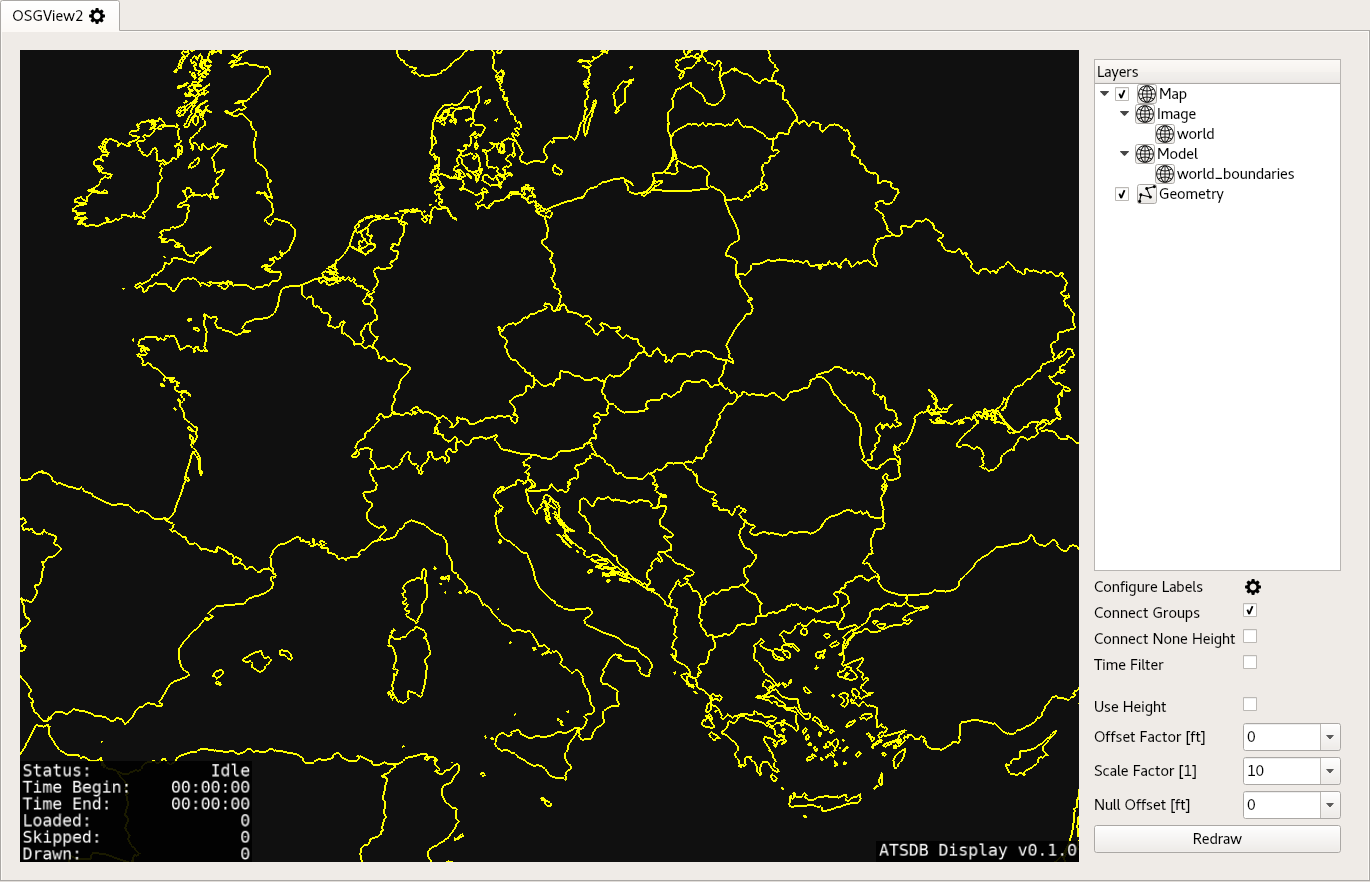
\includegraphics[width=18cm,frame]{../screenshots/osgview_overview.png}
  \caption{OSG View overview}
  \label{fig:osgview_overview}
\end{figure}

The map window will automatically traverse to the medium location of the data in the current database.

\subsubsection{Map Widget}
\label{sec:osgview_map}

In the map widget, several mouse and key operations are supported. The following terms are used:

\begin{itemize}
 \item LMB: Left mouse button
 \item MMB: Middle mouse button
 \item RMB: Right mouse button
 \item CTRL: CTRL key
\end{itemize}

\begin{table}[H]
  \center
  \begin{tabular}{ | l | l | l |}
    \hline
    \textbf{Mouse Action} & \textbf{Key Action} &  \textbf{Description} \\ \hline
    Single click & - & - \\ \hline
    LMB click \& drag & - & Traverse map \\ \hline
    - & Arrows & Traverse map \\ \hline
    MMB click \& drag & - & Rotate map \\ \hline
    RMB click \& drag & - & Zoom map \\ \hline
    MMB scroll \& drag & - & Zoom map \\ \hline
    LMB double click & - & Zoom to clicked location \\ \hline
    RMB double click \& drag & - & Zoom away from clicked location \\ \hline
    - & Space bar & Return to home position \\ \hline
  \end{tabular}
  \caption{Map widget view operations}
\end{table}

Further operations are defined in section Map Widget Data Operations.

\subsubsection{Configuration Widget}
\label{sec:osgview_config}

In the configuration widget, several elements exist:

\begin{itemize}
 \item Layer widget: displays all currently existing layers
 \item Height widget: configures if and how height information is used
 \item Time filter: De/activates the time window filter
\end{itemize}

\subsubsection{Layer Widget}

In the layer widget, a tree view is given to configure the display of the existing elements. The following main tree elements are:
\begin{itemize}
 \item Map: Shows current map layers
 \item Geometry: Shows current DBO elements
\end{itemize}

\subsubsection{Changing the Background Map}

Please note that, while the default background map is supplied ATSDB, the other background map types are downloaded from public Internet sources and therefore require an Internet connection. They are then cached locally to facilitate faster access. \\

To change the background map, click the globe symbol {
\includegraphics[scale=0.05]{../../data/icons/globe.png} in Map Layer to access the map selection. The following maps are commonly available:

\begin{itemize}
 \item arcgis.earth
 \item minimal.earth
 \item openstreetmap.earth
 \item readymap.earth
 \item readymap-detailed.earth
\end{itemize}

The map loading and display in based on the osgEarth library (\url{http://osgearth.org/}), as are to map file definitions. The map which can be set using this dialog is simply a file list from the folder '~/.atsdb/data/maps'. So, changes can be made to the supplied ones or custom user maps can be added to this folder. \\
Please refer to \url{http://docs.osgearth.org/en/latest/references/earthfile.html} for a definition of an earth file.

\newpage
\paragraph{ArcGIS Map}

As supplied in the osgEarth example files, this map data is obtained from ArcGIS Online (\url{https://doc.arcgis.com/en/arcgis-online/reference/what-is-agol.htm}). It shows satellite imagery, supplied with elevation data from ReadyMap. 

\begin{figure}[H]
    \hspace*{-2cm}
    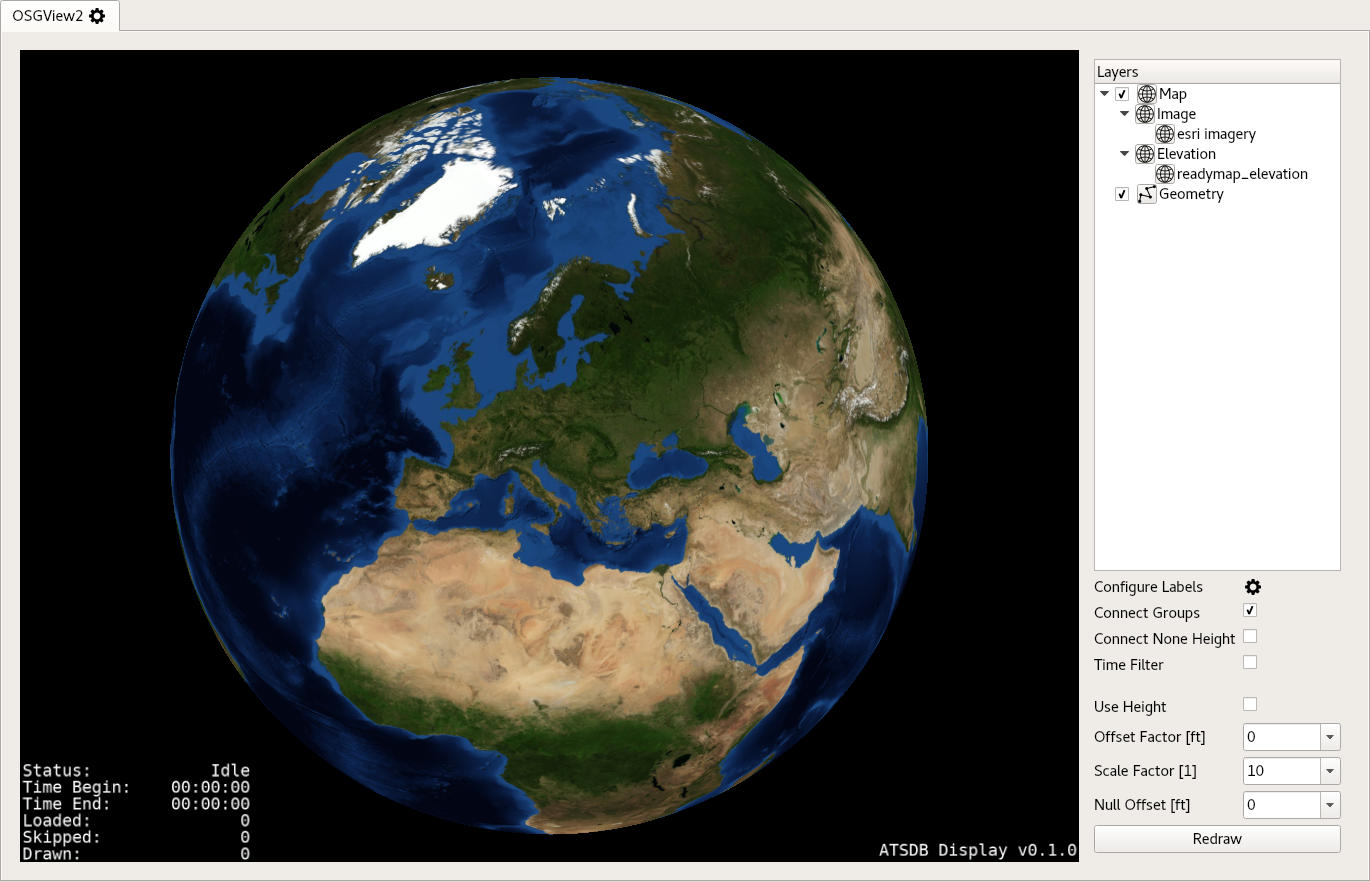
\includegraphics[width=18cm,frame]{../screenshots/osgview_arcgis.png}
  \caption{OSG View Arcgis map}
\end{figure}

\newpage
\paragraph{Minimal Map}

This minimal map shows national borders based on an ESRI shapefile, provided by Bjorn Sandvik on \url{thematicmapping.org}.

\begin{figure}[H]
    \hspace*{-2cm}
    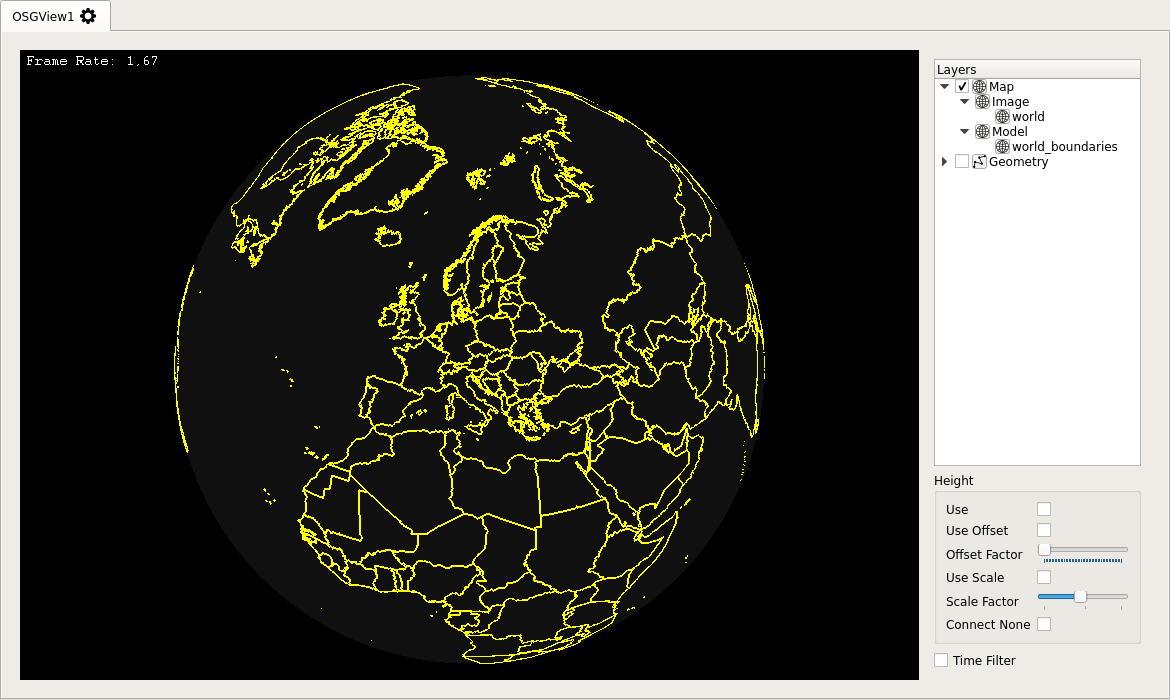
\includegraphics[width=18cm,frame]{../screenshots/osgview_minimal.png}
  \caption{OSG View minimal map}
\end{figure}

\newpage
\paragraph{Open Street Map}

This very useful map shows map data from \url{https://www.openstreetmap.org/}.

\begin{figure}[H]
    \hspace*{-2cm}
    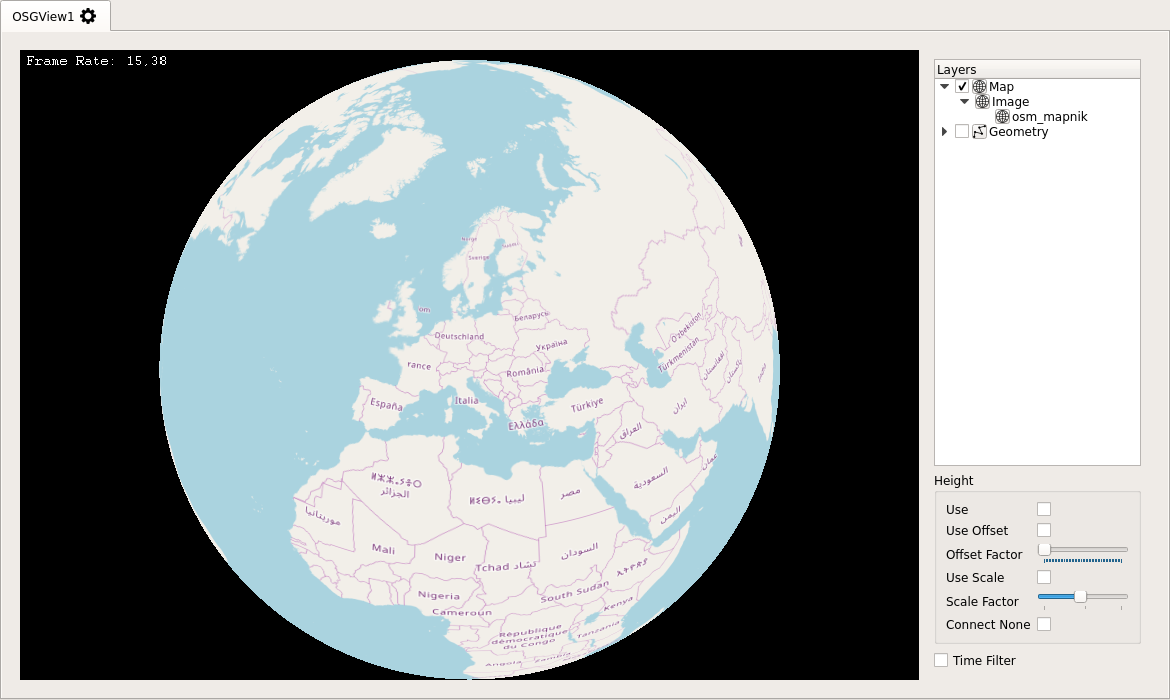
\includegraphics[width=18cm,frame]{../screenshots/osgview_osm.png}
  \caption{OSG View OpenStreetMap}
\end{figure}

It is possible to zoom in to a very high level of detail, to even inspect airport layouts.

\begin{figure}[H]
    \hspace*{-2cm}
    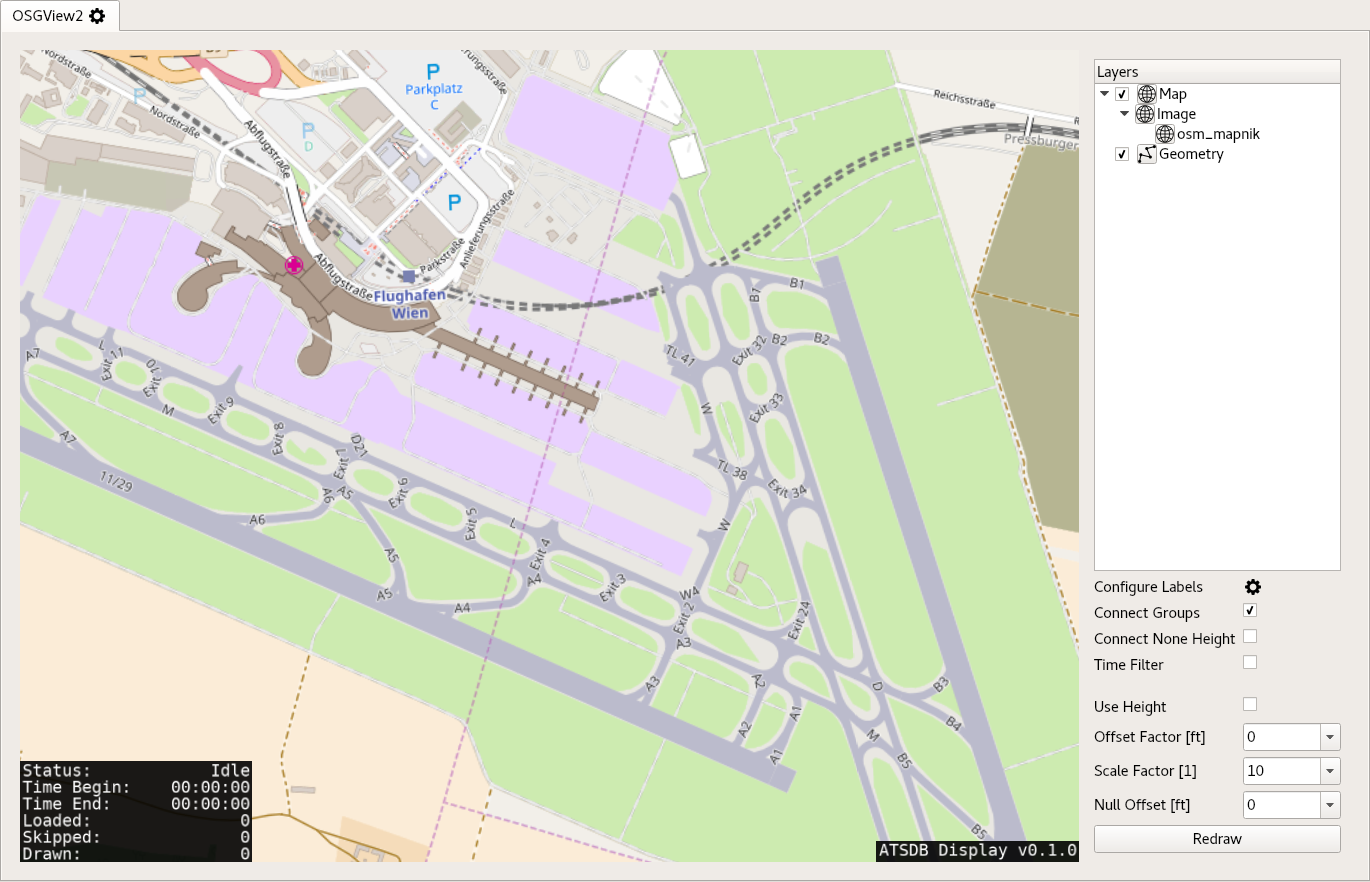
\includegraphics[width=18cm,frame]{../screenshots/osgview_osm_vienna.png}
  \caption{OSG View OpenStreetMap Vienna Airport}
\end{figure}

\newpage
\paragraph{ReadyMap}

This map also shows satellite data, from \url{http://web.pelicanmapping.com/readymap-tiles/}. It includes an elevation layer, so ground elevation is observable.

\begin{figure}[H]
    \hspace*{-2cm}
    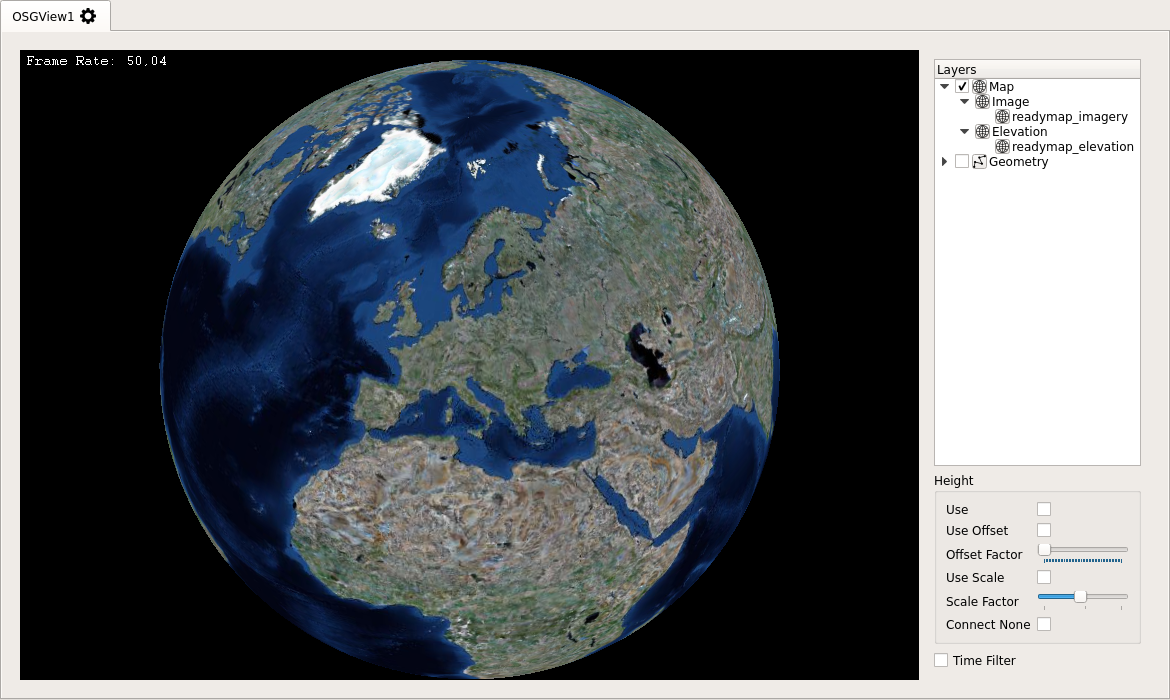
\includegraphics[width=18cm,frame]{../screenshots/osgview_ready.png}
  \caption{OSG View ReadyMap}
\end{figure}


\paragraph{ReadyMap Detailed}

This map shows the same data as ReadyMap, but to a higher detail level.

\begin{figure}[H]
    \hspace*{-2cm}
    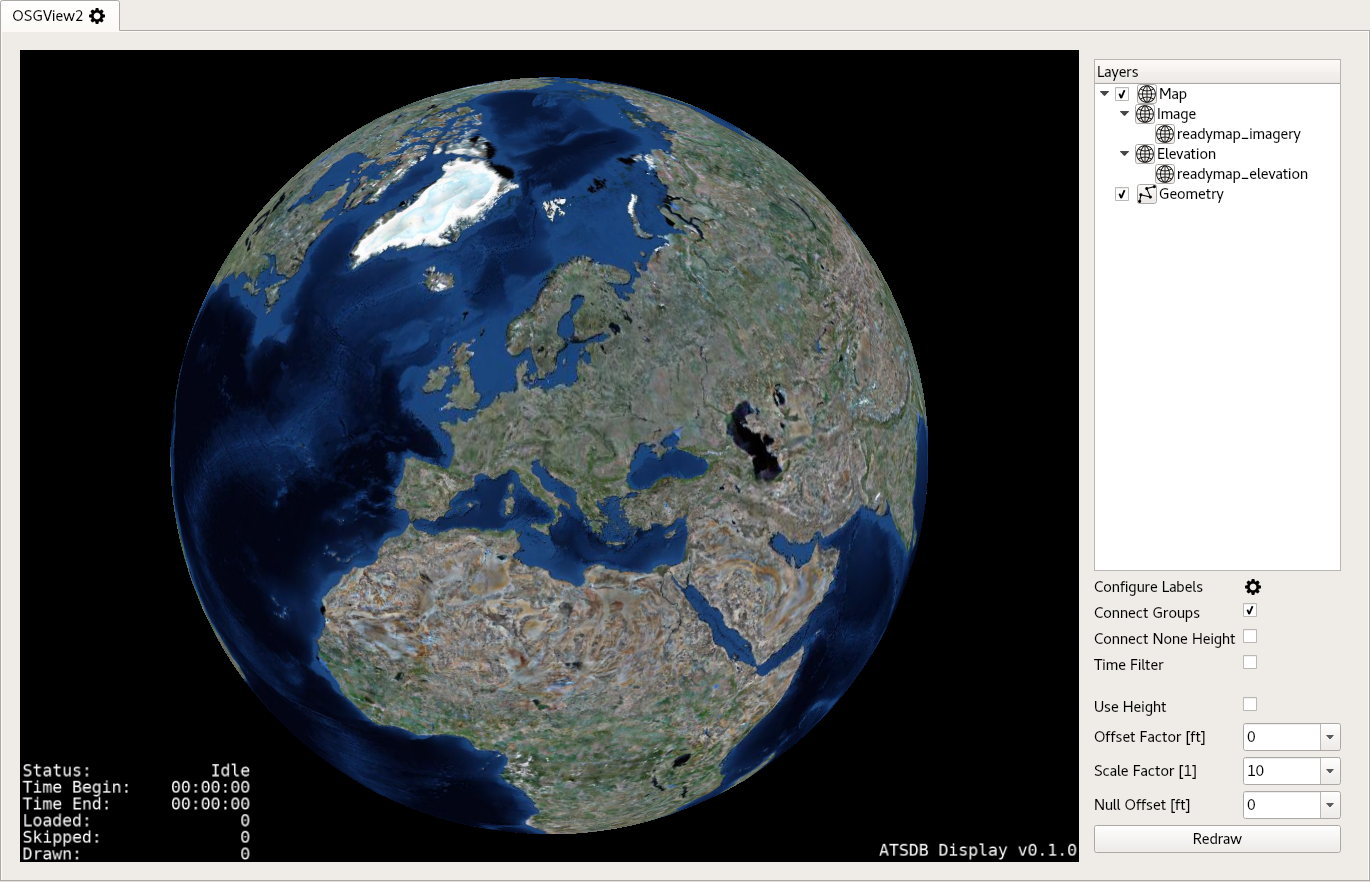
\includegraphics[width=18cm,frame]{../screenshots/osgview_ready_detail.png}
  \caption{OSG View ReadyMap detailed}
\end{figure}


\begin{figure}[H]
    \hspace*{-2cm}
    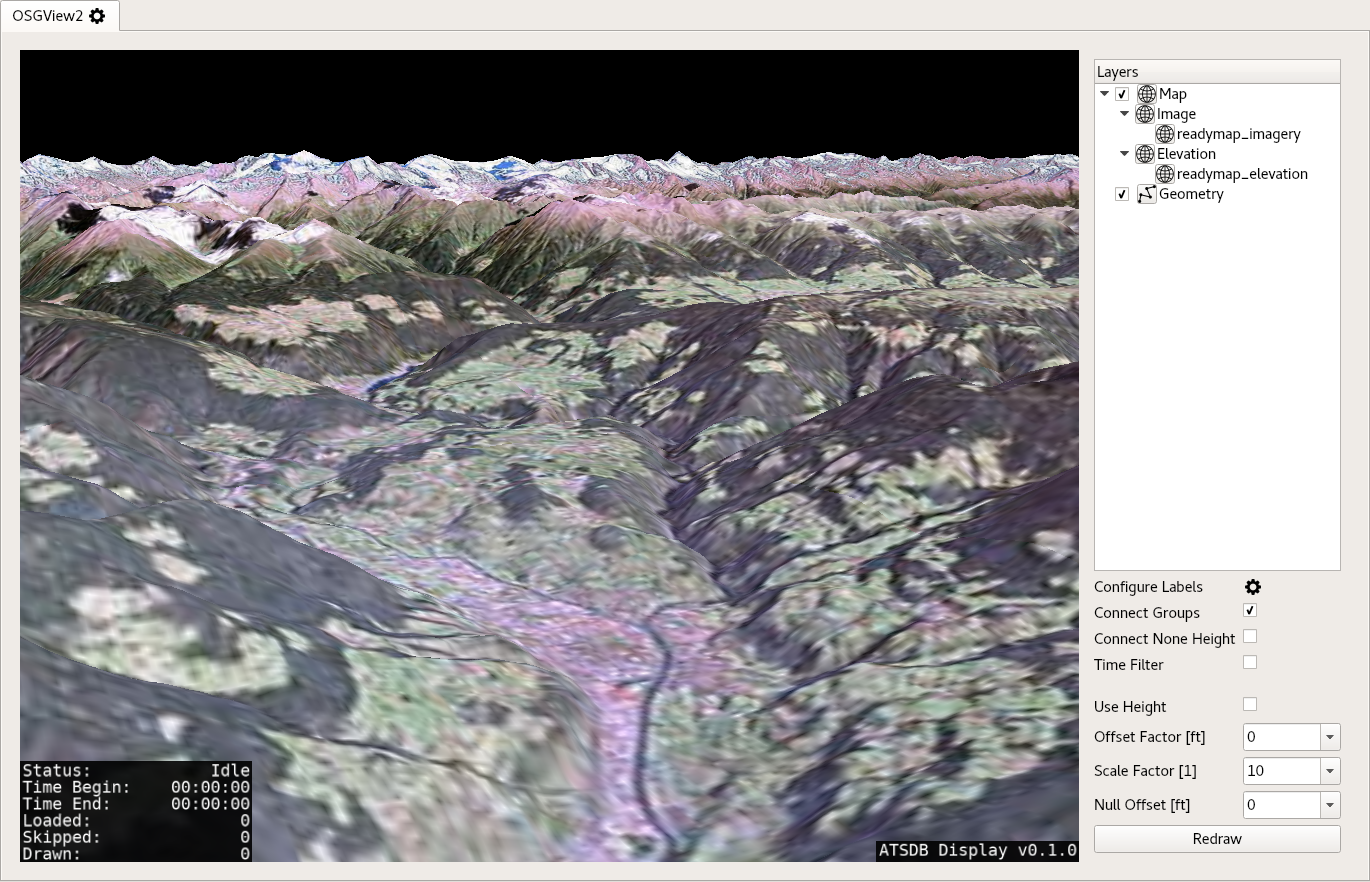
\includegraphics[width=18cm]{../screenshots/osgview_readymap_elav.png}
  \caption{OSG View ReadyMap detailed elevation}
\end{figure}


\subsubsection{Loading Data}
To load data, trigger a loading action from the Management widget. The data will be loaded as with the Listbox View, and displayed during the loading process. 

\begin{figure}[H]
    \hspace*{-2cm}
    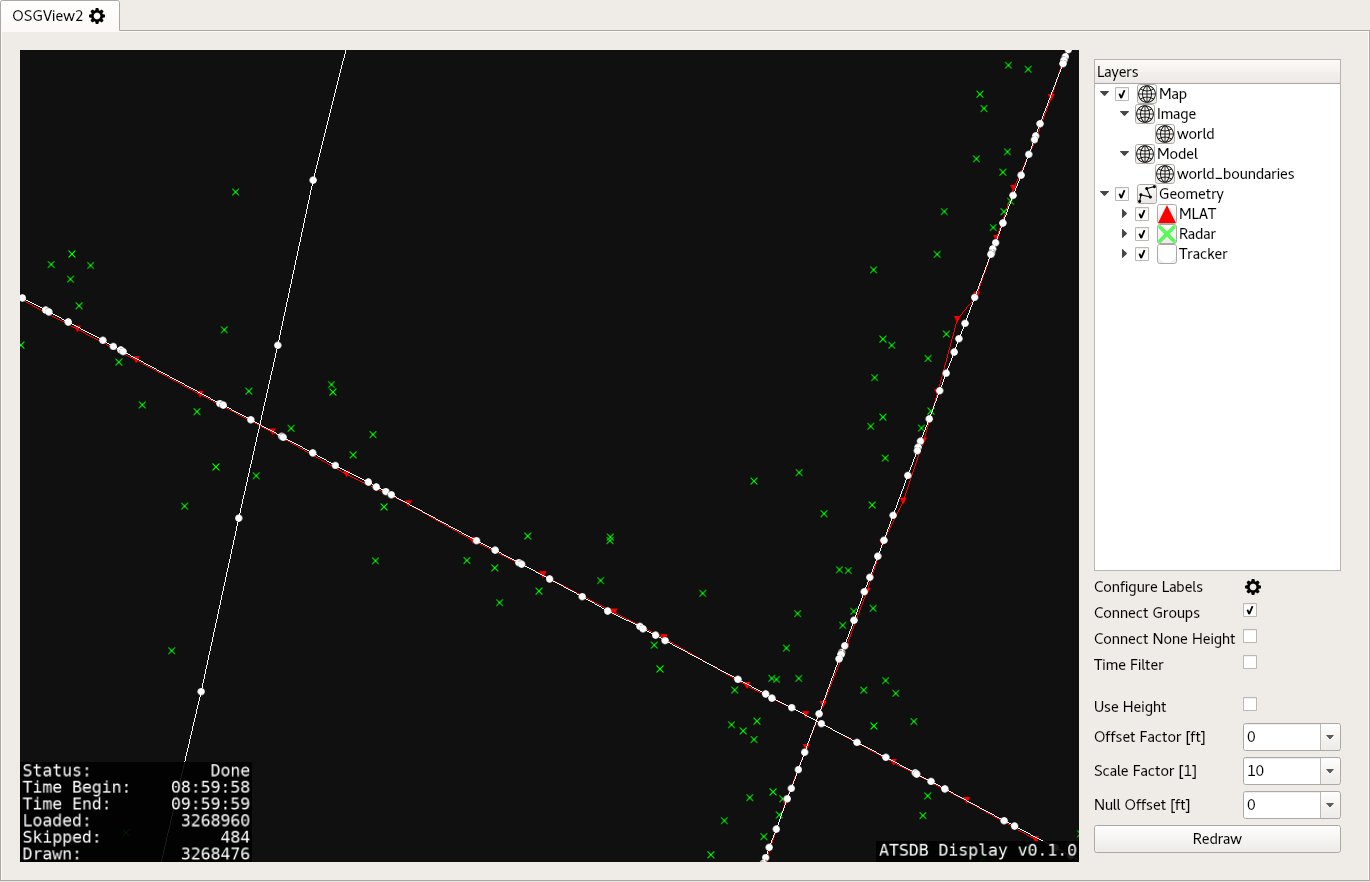
\includegraphics[width=18cm,frame]{../screenshots/osgview_data.png}
  \caption{OSG View data display}
  \label{fig:osgview_data}
\end{figure}

Please note that since currently only an example dataset is used, until real surveillance data can be made available.

Now, the loaded data is displayed in the following manner: For each DBO, a list of sensors exist, which supply the shown target reports. In the Geometry layers, the data is grouped as follows: Database Object $\rightarrow$ Sensor $\rightarrow$ Group. \\

For each DBO, a default display configuration is set:

\begin{itemize}
 \item ADS-B: Blue square
 \item MLAT: Red triangle
 \item Radar: Green cross
 \item Tracker: White circle
\end{itemize}

A sensor is of course a defined data source, e.g. a specific radar. A group currently is defined by a track number, and is connected by lines. If no track number is defined, the data is put into the 'Unassociated' group and not connected by lines.

\subsubsection{Layer Operations}

In the Layers widget, a number of operations are possible for each tree item.

\begin{table}[H]
  \center
  \begin{tabular}{ | l | l | l |}
    \hline
    \textbf{Operation} & \textbf{Trigger} &  \textbf{Description} \\ \hline
    View sub-items & Triangle & Opens or closes view of the sub-items \\ \hline
    Display item & Checkbox & Enables or disables display of items (and all sub-items) \\ \hline
    Display context menu & Click on symbol & Opens the items context menu \\ \hline
  \end{tabular}
  \caption{Layer operations}
\end{table}

The context menu allows several actions to be performed on an item. If an item has sub-items, the same action will automatically be performed on the child items.

\begin{figure}[H]
    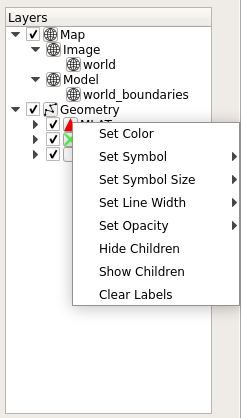
\includegraphics[width=5cm,frame]{../screenshots/osgview_layer_context_menu.png}
  \caption{OSG View layer context menu}
\end{figure}

\begin{itemize}
 \item Set Color: Open colour dialog to set the items colour
 \item Set Symbol: Set the items symbol to one of the following values:
\begin{itemize}
 \item Cross
 \item Circle
 \item Square
 \item Triangle
\end{itemize}
 \item Set Symbol Size: Set the symbols size
 \item Set Line Width: Set the line width
 \item Set Opacity: Set the items opacity
 \item Hide children: Disable display off all children
 \item Show Children: Enable display of all children
 \item Clear Labels: Removes all labels
\end{itemize}

Please note that only the main Map item has a context menu, and only allows setting of map files and changing the opacity.

\subsubsection{Map Widget Data Operations}
\label{sec:osgview_data_operations}

Several data-related operations can be also performed in the map widget.

\begin{table}[H]
  \center
  \begin{tabular}{ | l | l | l |}
    \hline
    \textbf{Mouse Action} & \textbf{Key Action} &  \textbf{Description} \\ \hline
    LMB click & CTRL & Toggle label display of a single target report \\ \hline
    RMB click & CTRL & Show data context menu \\ \hline
  \end{tabular}
  \caption{Map widget data operations}
\end{table}

Label display is currently somewhat limited, but shows the following attributes:

\begin{itemize}
 \item C: Mode C code in feet, if available
 \item A: Mode A code (octal), if available
 \item CS: Mode S target indentification, if available
 \item R: Record number in database
 \item TA: Mode S target address (hexadecimal), if available
 \item T: Time of day (HH:MM:SS.SSS)
 \item TN: Track number, if available
\end{itemize}

Also, the label colour is always the same as the target report's.

\begin{figure}[H]
    \hspace*{-2cm}
    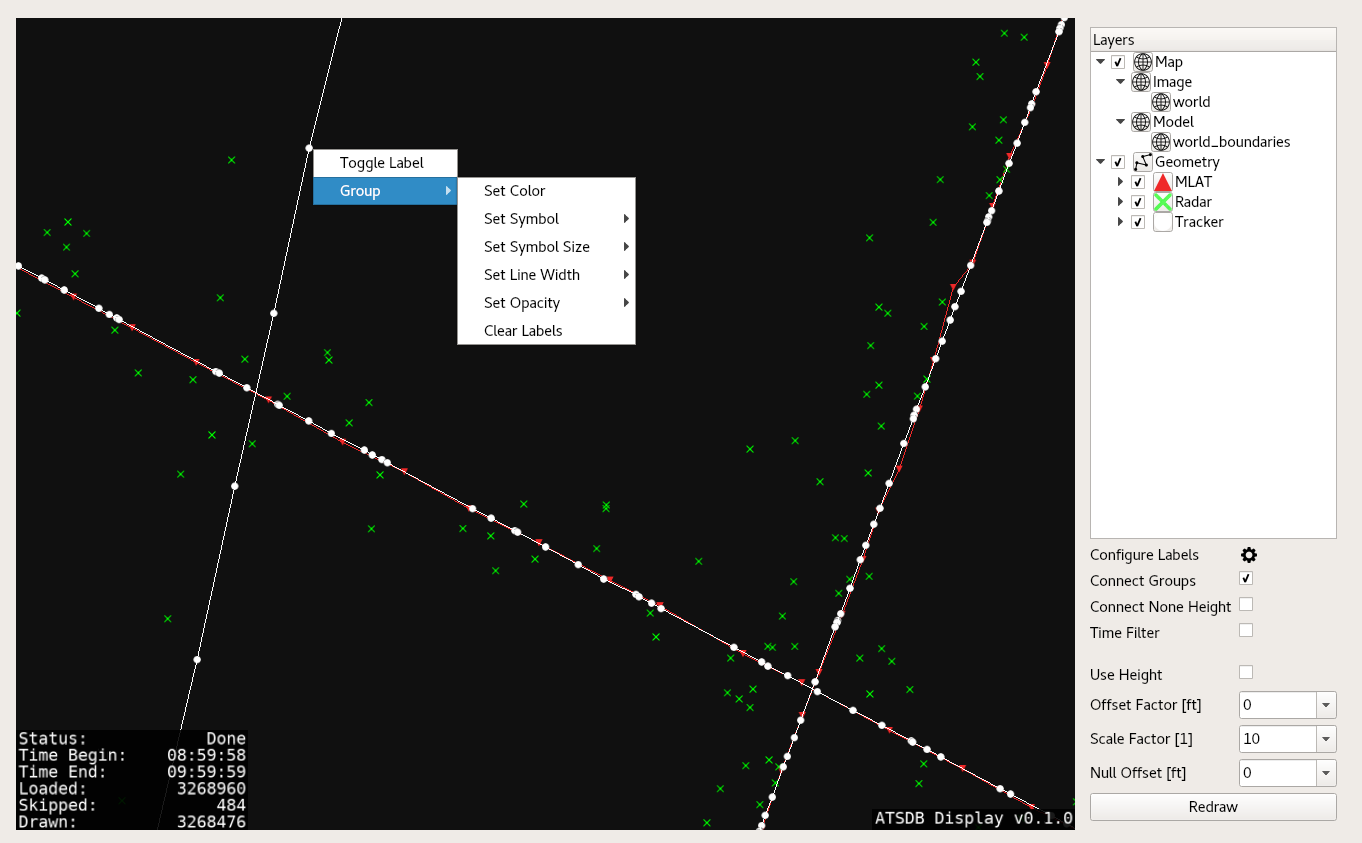
\includegraphics[width=18cm,frame]{../screenshots/osgview_data_operations.png}
  \caption{OSG View data operations}
\end{figure}

The data context menu allows the following operations:

\begin{itemize}
 \item Toogle Label: Toggle label display of a single target report
 \item Group: Same operations as on the item's group layer item
\end{itemize}

\subsubsection{Height Operations}

Per default, a target reports height is not used for display, which is common in current air-traffic displays. However, in certain situation a true 3D display might be of interest to a user, and therefore several options where incorporated:

\begin{itemize}
 \item Use: Use the height based on Mode C $h_c$, transformed to meters
 \item Use Offset: Whether to use an additative height offset
 \item Offset Factor: Height offset value $h_o$
 \item Use Scale: Whether to use an multiplicative factor
 \item Scale Factor: Height scale factor value $h_s$
 \item Connect none: Whether to draw lines to target reports with no height information
\end{itemize}

Generally, if no height information is given (no Mode C code), the height is either $0$ or the height offset (if used). That means that those target reports appear to the on the ground. If connection lines are drawn between the ones in the air and those without, a lot of annoying lines are shown.

The formula to calculate the height is as follows:

$$ h = h_o + h_s \cdot h_c [m]$$ 

Please note that upon changes to the height usage, the complete geometry data is redrawn, which can take several seconds until complete.

\subsubsection{Time Filter}

Once activated, the time filter facilitates that only target reports within a specific time window are shown.


\begin{figure}[H]
    \hspace*{-2cm}
    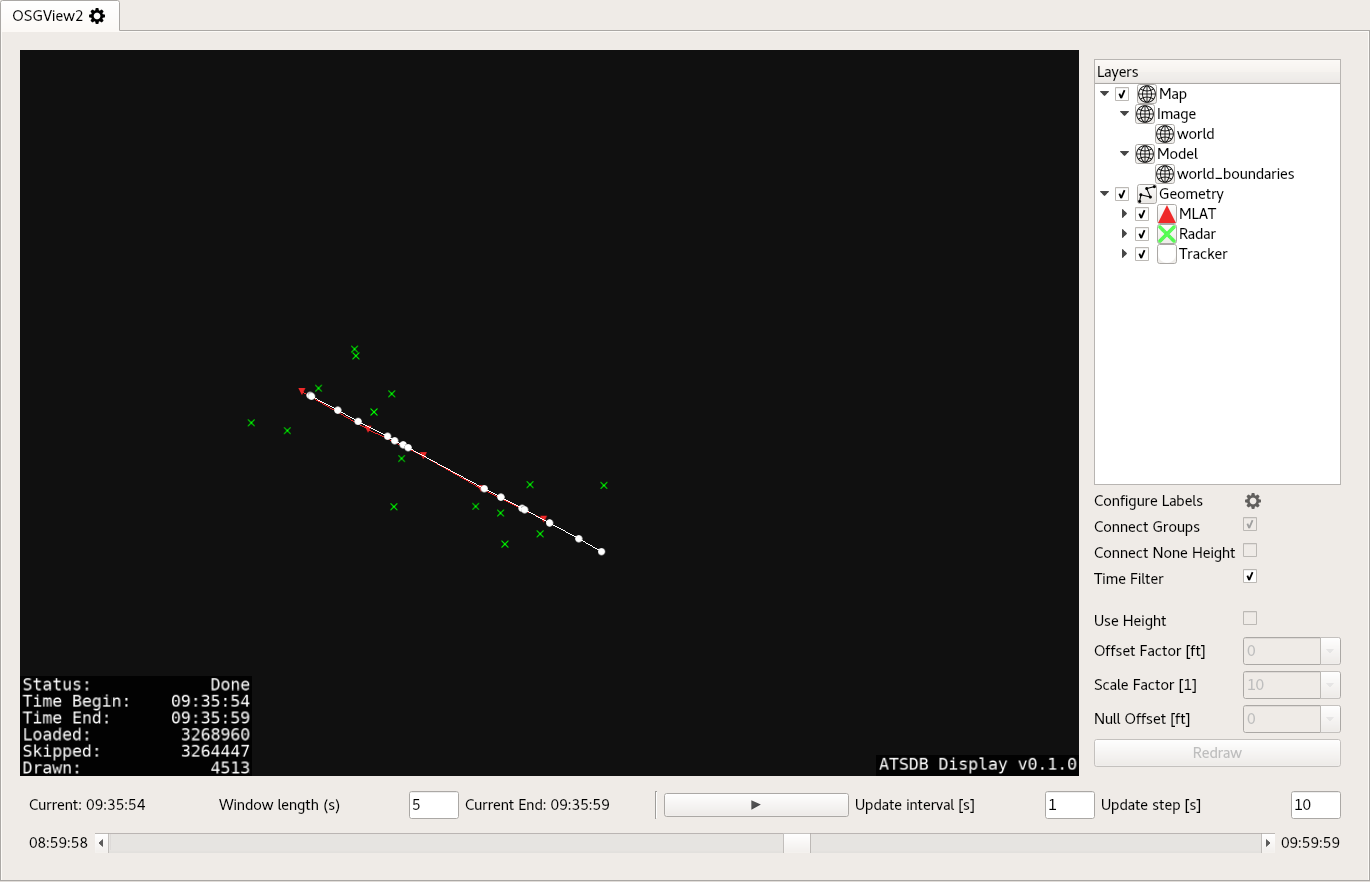
\includegraphics[width=18cm,frame]{../screenshots/osgview_time_filter.png}
  \caption{OSG View time filter}
  \label{fig:osgview_time_filter}
\end{figure}

The following items exist:

\begin{itemize}
 \item Current: The start of the time window
 \item Window length (s): Duration of the display time window
 \item Current End: The end of the time window
 \item Play button: Start/Stop the auto-play mode
 \item Update interval [s]: Auto-play mode update interval
 \item Update step [s]: Auto-play mode update step
 \item Scrollbar: Manual time-scrolling
\end{itemize}

Please note that unfortunatly in the AppImage especially the time filtering is slower than was to be expected. This is currently under investigation.
 
